\chapter[Networking]{Networking \\ \Large \textnormal{Marc Dufay}}

This individual milestone focuses on implementing networking capabilities in order to communicate with other devices. This is done by implementing a driver to be able to send and receive network packet from the Ethernet port, then parsing and crafting these packets to support multiple protocols, such as ARP, ICMP or UDP.

\section{Driver}

\subsection{Network device}

There are two drivers implemented to use networking capabilities on the OS:
\begin{itemize}
\item A Virtio-net driver for the virtual network device available with Qemu
\item An Enet driver available for the Toradex board
\end{itemize}

The operating system has support for these two drivers and will use the one matching the platform.

To be able able to use the driver, we need to have an access to the physical memory range used by the device, this is done using the \verb|dev_cap| capability and the following code:

\begin{lstlisting}
struct capref dev_cap = { .cnode = cnode_task, .slot = TASKCN_SLOT_DEV };
struct capability dev_frame;
errval_t err = cap_direct_identify(dev_cap, &dev_frame);
if (err_is_fail(err) || dev_frame.type != ObjType_DevFrame) {
   DEBUG_ERR(err, "cap_direct_identify");
   return err;
}
err = dev_frame_map(dev_cap, dev_frame, IMX8X_ENET_BASE, IMX8X_ENET_SIZE, (void**)&st->d_vaddr);
if (err_is_fail(err)) {
   return err;
}
\end{lstlisting}

The driver initialization is done in the following order:
\begin{itemize}
\item Map the device memory region
\item Check for the device response and enable it
\item Configure the device and wait for it to be ready to send/receive packet
\item Retrieve the MAC address of the device
\item Initialize the transmit and receive queue
\end{itemize}

\subsection{Network driver}

The given driver does not support interrupts. Thus to be able to process network packets with low latency, we need to be constantly polling for new packet. We do so by running the driver on a separate process. This driver does the bare minimum in term of networking: it supports receiving and sending network packets. Everything else is handled by the network handler running in the init process.
\medskip

After being initialized, the driver stays in the following loop:
\begin{lstlisting}
while(true){
   err = check_for_event(ws);
   if(err_is_ok(err)){
       err = event_dispatch(ws);
       assert(err_is_ok(err));
   }
   receive_packet();
   thread_yield();
}
\end{lstlisting}
Basically we are alternating between checking for packets to send, sending them (\verb|check_for_event| and \verb|event_dispatch|) and checking for packets to receive (\verb|receive_packet|). The packets to send are sent by the network handler in the init process and as soon as we receive a packet, it is also forwarded to the network handler. Then we yield the thread in order not to starve other processes. This loop is need as the driver does not support interrupts.

\subsection{Network queue}

Barrelfish provides an abstraction over the process of sending/receiving packets in the form of device queues. Device queues (\verb|struct devq|) represent the packet send/receive queues. They have the same interface for any driver we are using, the difference being the size of the queue can vary depending on the device. The device queue provide the following interface:

\begin{itemize}
\item \verb|devq_register|: Register a given frame to be used inside the queue. The process keeps ownership of the memory inside this frame.
\item \verb|devq_enqueue|: Give ownership of a given memory region to the device. For a receive queue, this makes the memory range ready to receive a packet. For the transfer queue, this makes the device send a packet whose data is what is contained in the valid memory region enqueued by this call.
\item \verb|devq_dequeue|: Get back ownership of a memory range. For a receive queue, if this calls did not fail, it means we received a packet in the valid region of the memory range. For the transfer queue, we use it to get back ownership after a packet was sent and the device no longer needs this memory.
\end{itemize}

For the transfer queue, we keep a boolean array for which part of the region (divided in packet of 2048 bytes as that is an upper bound on the maximum size of one packet) is ready to be used to send one packet.

\section{Asynchronous communication}

Networking is by its use asynchronous. We don't know when we receive a packet and the driver must be able to send a packet at any time to minimize latency. This causes issues with our current way of communication in a single core: it only supports communications from a process to its init process and is blocking (no other communication can be sent before a response has been received). As such, it is not suited for networking.

\medskip

To solve this issues, we can add an additional layer on top of the existing rpc to make it asynchronous, two ways and not blocking. However, this would prevent us from using the underlying rpc layer, which is still needed for all other rpc calls. The solution is for processes using the network (this includes the driver) to create a secondary lmp channel between them and the init process. Then we make this lmp channel asynchronous in order not to disturb the primary lmp channel. This allows for two-way non-blocking exchanges between a process and the network handler, needed by the driver and for processes having a UDP/TCP server.

\section{Mac address resolution}

Every packet starts with an Ethernet header, which contains the source MAC address and the destination MAC address. We should always know one of the two which should be our own MAC address (or the broadcast FF.FF.FF.FF.FF.FF MAC address). However, when communication we mostly address devices using their IP. Therefore we need to be able to get a device MAC Address using its IP. This can be done using an ARP (Address resolution protocol) packet. The device looking to get the MAC broadcast an ARP request with the given IP and the device with this IP responds with its MAC address.

\begin{figure}
    \centering
    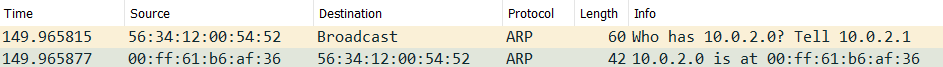
\includegraphics[scale=0.6]{images/network/arp_request.png}
    \caption{An ARP request done by the OS, observed by WireShark}
\end{figure}

\subsection{Receiving an ARP packet}

An ARP packet has the following layout:


When we receive an ARP request to our given IP, we craft a response packet with our MAC address and immediately send it back.

\begin{lstlisting}[caption={Sending back an ARP response}]
if (arp_header->ip_dst == self_ip) {
    // respond to the request
    const size_t packet_rep_size = sizeof(struct eth_hdr) + sizeof(struct arp_hdr);
    uint8_t     *packet_rep_data = malloc(packet_rep_size);
    _make_ETH_header(packet_rep_data, arp_header->eth_src, ETH_TYPE_ARP);
    _make_ARP_header(packet_rep_data + sizeof(struct eth_hdr), arp_header->eth_src,
                     arp_header->ip_src, ARP_OP_REP);
    simple_async_request(ns.async, packet_rep_data, packet_rep_size, async_request_free,
                         NULL);
}
\end{lstlisting} 

\subsection{Sending an ARP packet}

In order to send an ARP packet, we set its destination to the special MAC address FF.FF.FF.FF.FF.FF meaning we broadcast it. The request is then saved to a doubly linked list, along with the target IP. This way, when we receive an ARP response, we look at the linked list, find any request it can match and satisfy them.

\subsection{Dealing with timeouts}

Of course, if we send a request to an IP which does not exist, we will never get an answer. To deal with this, for each request, we set an associated \verb|deferred_event| which after a given time (5 seconds for an ARP request) will trigger, cause the item to be removed from the doubly linked list and a \verb|NETWORK_ERR_IP_RESOLVE_TIMEOUT| error to be returned.

\begin{lstlisting}[caption={dealing with timeouts}]
static void _network_arp_timeout(void *arg)
{
    struct request_with_timeout *req = arg;
    // remove it from the list
    req->next->prev = req->prev;
    req->prev->next = req->next;

    *req->err = NETWORK_ERR_IP_RESOLVE_TIMEOUT;
    req->resume_fn.handler(req->resume_fn.arg);
    free(req);
}
\end{lstlisting}  

This method is of course used for any request made, to make sure we are not stuck waiting for a response. If we get a response, we cancel the deferred event using \verb|deferred_event_cancel|.

\subsection{IP to MAC cache}

We want to minimize the number of requests done, as such it is inefficient to query the MAC of an IP address if we already have a way to get it. To fix this issues, the network handler has an IP to MAC cache.
\begin{lstlisting}
// hash table containing the ip to mac addresses we received
collections_hash_table *ip_to_mac;
\end{lstlisting}
This cache is done using a hash table. An IP can be represented as a 32-bit integer and is the key in this hash table to find the MAC address. Every time we receive an ARP or IP packet, we get access to the IP and MAC address of the sender and store it.

\section{Ping support}

Next is the support for the ping command, this commands relies on the ICMP (Internet Control Message Protocol) packet, the client sends an echo request and the target sends a reply with data of the request to prove it received it.

\begin{figure}
    \centering
    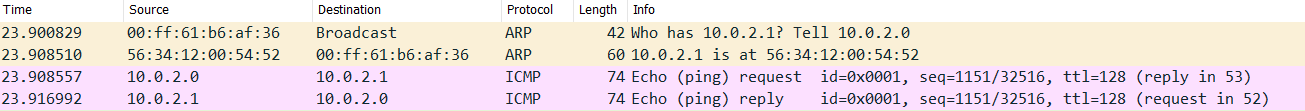
\includegraphics[scale=0.45]{images/network/ping_request.png}
    \caption{A ping request to the OS, observed by WireShark}
\end{figure}

\subsection{Receiving a ping request}

When we receive a PING request, we can immediately reply to it. The ICMP packet (and the above IP packet) are more complex, they require a checksum to check the integrity of the packet, which is the bitwise not of the added 16-bit values of the packet with carry.

An ICMP packet also has two identifiers and a payload which we need to send back to prove that we have correctly received the packet.

\begin{lstlisting}[caption={Replying to an ICMP packet}]
const uint16_t ip_packet_res_size    = sizeof(struct ip_hdr) + packet_size;
const uint16_t total_packet_res_size = sizeof(struct eth_hdr) + ip_packet_res_size;
uint8_t       *res_packet            = malloc(total_packet_res_size);
_make_ETH_header(res_packet, src_mac, ETH_TYPE_IP);
_make_IP_header(res_packet + sizeof(struct eth_hdr), src_ip, ip_packet_res_size,
                IP_PROTO_ICMP);
_make_ICMP_header(res_packet + sizeof(struct eth_hdr) + sizeof(struct ip_hdr), packet_size,
                  icmp_header->payload, ICMP_ER, ntohs(icmp_header->id),
                  ntohs(icmp_header->seqno));
\end{lstlisting}

\subsection{Sending a ping request}

Sending a ping request is more complex as we may need to make an ARP request, it has the following scheme:
\begin{itemize}
\item Serialize the request, if we already have the MAC address, skip the next step
\item Compute the current timestamp, send an ARP request and put the request in the ARP list. If we get a timeout, return immediatly.
\item Generate the payload, send the ICMP request and put the request in the ping list.
\item If we get a timeout, return \verb|NETWORK_ERR_REQUEST_TIMEOUT|.
\item Otherwise, compute the time the ping request took and send it back.
\end{itemize}

For each new ping request, we have a different identifier and generate a different payload (containing only lowercase english characters). When we receive the request, we check that the identifier and payload matches.

\section{UDP support}

The UDP protocol is really simple, it adds a source port and destination port but is much simpler than the ICMP packet. The difficulty lies in setting an easy to use UDP server for a process.

\subsection{Interface}

The network library comes with a header \verb|network.h| in aos which can be used by any process to do network requests:
\begin{lstlisting}[caption={network.h interface}]
errval_t network_init(void);

errval_t ping(uint32_t target_ip, uint32_t* ping_ms);

errval_t network_listen(uint16_t port, enum server_protocol protocol, network_listener listener, void* meta);

errval_t network_send(uint32_t ip, uint16_t port, enum server_protocol protocol, uint16_t src_port, uint16_t data_size, void* data);
\end{lstlisting}

Network init is used to setup some internal structures which we will talk about and setup the secondary asynchronous channel if it was not already setup. 

\subsection{UDP server}

The UDP server is divided in two parts. First each process has a singly linked list containing a port and the callback to call.
\begin{lstlisting}
struct listener_list{
    struct listener_list* next;
    enum server_protocol protocol;
    uint16_t port;
    network_listener listener;
    void* meta;
};
\end{lstlisting} 

Then the init process containing the network handler has a hashmap, containing for each port the process id which is listening to it (if there is one).

\begin{lstlisting}
errval_t network_register_listen(uint16_t port, bool is_tcp, domainid_t pid){
    uint64_t key = port * 2ULL + is_tcp;
    if (collections_hash_find(ns.port_to_pid, key) != NULL)
        return NETWORK_ERR_PORT_ALREADY_USED;

    collections_hash_insert(ns.port_to_pid, key, (void*)(uint64_t)pid);

    return SYS_ERR_OK;
}
\end{lstlisting}

This way when we received a UDP request, the following happens:
\begin{itemize}
\item Look in the network handler hash table if there is a process listening to it, if not return.
\item Craft a request to the given PID, if in the same core, send it immediately using its async channel. Otherwise, send it to the appropriate core.
\item The process looks in its linked list for the callback to call given the port, then calls it.
\end{itemize}


\subsection{Remote Shell}

Using UDP packet, we can now implement a shell over the network. This remote shell is using UDP packet, meaning some packets can be lost. To do so, a new shell command \verb|setio| is added to define whether to use serial or network io. And for network io which remote ip, port and host port to use.

\medskip

The \verb|getchar| and \verb|putchar| functions are then intercepted in the RPC handler and the network version of these functions are used if enabled. We also look when receiving a UDP packet if it matches the parameters of the remote shell and if so use its content for serial io.

\begin{figure}[H]
    \centering
    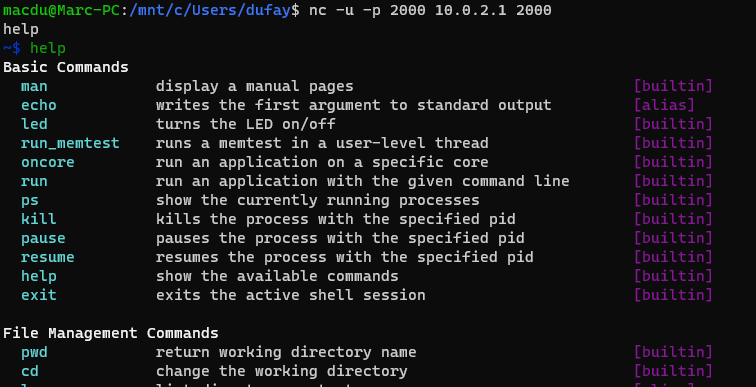
\includegraphics[scale=0.75]{images/network/network_io.png}
    \caption{Using netcat as a shell for our OS}
\end{figure}

\section{Performance}

\begin{figure}
    \centering
    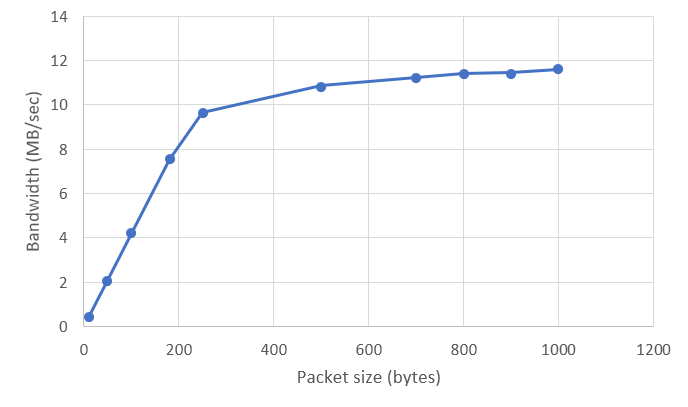
\includegraphics[scale=0.7]{images/network/graph-perf.png}
    \caption{Bandwidth recorded using the enet driver, depending on the packet size}
    \label{fig:enter-label}
\end{figure}

To test the implementation, a stress test was done by sending as many UDP packets of a given size as possible in a given time range. The UDP packet were crafted and sent by a C++ program using boost asio. When the packet is greater than 500 bytes, no packet loss was recorded. The smaller the packet was, the bigger the percentage of packet loss became, with 50\% packet loss using packets of 10 bytes.

\medskip

Furthermore, it appears that the driver has a hard limit of around 42.5 thousands packets per second, which is reached for packets of size less than 200 bytes. The maximum bandwidth recorded was almost 12 MB/sec, reached with the biggest packet size (packets bigger than 1000 bytes were getting fragmented). About latency, performing 100 ping request and taking the average, we get a value of 5ms, which means packets have a 2.5ms latency in average.

\section{Retrospective}

Networking is by nature asynchronous, which is complex to implement in an operating system with a language like C which does not allow lambda or asynchronous operators. Building an architecture that supports well this asynchronous aspect and did not block at any time was the hardest part of this milestone and took a lot of planning.

The fact that the driver does not support interrupts makes also the driver not efficient, as it must always poll for new packets in order to minimize latency.